\documentclass[10pt,journal,compsoc,onecolumn]{IEEEtran}
\usepackage[utf8]{inputenc}
\usepackage{amsmath,amsfonts,amssymb}
\usepackage{amsthm}
\usepackage{graphicx}
\usepackage{cite}
\usepackage{textcomp}
\usepackage{tikz}
\usetikzlibrary{arrows,positioning,shapes.geometric}
\usepackage{booktabs}
\usepackage{url}

\newtheorem{theorem}{Theorem}
\newtheorem{lemma}[theorem]{Lemma}
\newtheorem{definition}[theorem]{Definition}
\newtheorem{corollary}[theorem]{Corollary}

\begin{document}

\title{Binary Search Trees: A Formal Analysis of Search, Insertion, Deletion, Construction, and Validation Algorithms}

\IEEEtitleabstractindextext{%
\begin{abstract}
The Binary Search Tree (BST) is a foundational data structure that enforces an ordering invariant to enable efficient search, insertion, and deletion. This paper presents a rigorous formal analysis of seven fundamental BST operations: (1) BST property identification and the distinction between local and global invariant checking; (2) Search, which exploits the ordering invariant for binary-search-style element location; (3) Insertion at leaf positions while preserving the BST property; (4) Finding minimum and maximum elements via leftmost and rightmost traversal; (5) Deletion covering all three cases (leaf, one child, and two children with inorder successor replacement); (6) Construction of a height-balanced BST from a sorted array using divide-and-conquer; and (7) BST validation via both inorder traversal sorting checks and the superior min-max range propagation approach. For each operation, we provide complete Java implementations, formal correctness proofs by structural induction, detailed dry-run trace tables, TikZ-rendered tree diagrams, and comprehensive complexity analyses. All core operations achieve O(H) time complexity where H is the tree height, motivating the study of self-balancing variants such as AVL and Red-Black trees.
\end{abstract}

\begin{IEEEkeywords}
binary trees, algorithms, data structures, computational complexity, tree traversal, recursive algorithms, formal analysis
\end{IEEEkeywords}
}

\maketitle
\IEEEdisplaynontitleabstractindextext
\IEEEpeerreviewmaketitle

\section{Introduction}
\label{sec:intro}

The Binary Search Tree (BST) is one of the most fundamental and widely-used data structures in computer science. By enforcing a simple ordering invariant --- every node in the left subtree holds a value strictly less than the node, and every node in the right subtree holds a value strictly greater --- BSTs enable efficient searching, insertion, and deletion operations that mirror the logic of binary search on sorted arrays, but with the flexibility of a linked, pointer-based structure.

BSTs find applications across a wide spectrum of computing:
\begin{itemize}
    \item \textbf{Database indexing:} B-trees and B$^+$-trees (generalizations of BSTs) form the backbone of database index structures, enabling logarithmic-time lookups on disk.
    \item \textbf{Symbol tables:} Compilers and interpreters use BSTs (or their balanced variants) to maintain symbol tables mapping identifiers to their types and memory locations.
    \item \textbf{File systems:} Directory structures often employ tree-based indexing for fast file lookup.
    \item \textbf{Priority queues:} Augmented BSTs support dynamic order-statistic queries and priority-based scheduling.
    \item \textbf{Autocomplete systems:} Trie-BST hybrids power real-time search suggestions.
\end{itemize}

This paper provides a rigorous formal analysis of seven fundamental BST operations:

\begin{enumerate}
    \item \textbf{BST Property and Validation (\S\ref{sec:property}):} Formal definition of the BST invariant and methods to verify whether a binary tree satisfies it.
    \item \textbf{Search (\S\ref{sec:search}):} Locating a target value by exploiting the ordering invariant.
    \item \textbf{Insertion (\S\ref{sec:insert}):} Adding a new value while preserving the BST property.
    \item \textbf{Finding Minimum and Maximum (\S\ref{sec:minmax}):} Exploiting the structure to locate extremal elements.
    \item \textbf{Deletion (\S\ref{sec:delete}):} Removing a node while maintaining the BST invariant, covering all three cases (leaf, one child, two children).
    \item \textbf{Constructing a Balanced BST from a Sorted Array (\S\ref{sec:construct}):} Building an optimally balanced BST using divide-and-conquer.
    \item \textbf{BST Validation (\S\ref{sec:validate}):} Two approaches --- inorder traversal and min/max range checking --- to verify the BST property.
\end{enumerate}

For each operation, we provide complete Java implementations, formal correctness proofs, detailed dry-run analyses with TikZ-rendered tree diagrams, and rigorous complexity analyses.

\section{Preliminaries}
\label{sec:prelim}

\subsection{Binary Tree Node Structure}

\begin{verbatim}
class TreeNode {
    int data;
    TreeNode left;
    TreeNode right;

    TreeNode(int x) {
        data = x;
        left = null;
        right = null;
    }
}
\end{verbatim}

\subsection{Formal BST Definition}

\begin{definition}[Binary Search Tree]
A binary tree $T$ is a \emph{Binary Search Tree} if and only if for every node $v \in T$:
\begin{enumerate}
    \item All nodes $u$ in the left subtree of $v$ satisfy $u.\text{data} < v.\text{data}$.
    \item All nodes $w$ in the right subtree of $v$ satisfy $w.\text{data} > v.\text{data}$.
    \item Both the left and right subtrees of $v$ are themselves BSTs.
\end{enumerate}
All node values are assumed to be \emph{distinct}.
\end{definition}

\begin{definition}[Height of a BST]
The \emph{height} $h$ of a BST with $N$ nodes satisfies:
\[
\lceil \log_2(N+1) \rceil - 1 \leq h \leq N - 1
\]
The lower bound is achieved by a perfectly balanced BST; the upper bound by a completely skewed (degenerate) BST.
\end{definition}

%% ============================================================
\section{BST Property and Visual Identification}
\label{sec:property}

\subsection{Common Misconception}

A frequent error is checking only the immediate children of each node: ``is $v.\text{left}.\text{data} < v.\text{data}$ and $v.\text{right}.\text{data} > v.\text{data}$?'' This is \emph{insufficient}.

\begin{figure}[htbp]
\centering
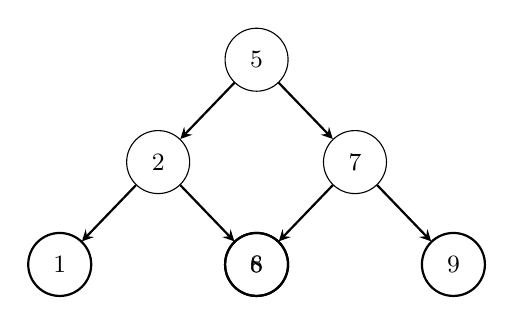
\begin{tikzpicture}[
  every node/.style={circle, draw, minimum size=0.8cm, font=\small, inner sep=1pt},
  level distance=1.3cm,
  sibling distance=2.5cm,
  edge from parent/.style={draw, ->, >=stealth, thick}
]
\node {5}
  child { node {2}
    child { node {1} }
    child { node {8} }
  }
  child { node {7}
    child { node {6} }
    child { node {9} }
  };
\end{tikzpicture}
\caption{\textbf{NOT a BST} despite each node satisfying the local child check. Node 8 is in the left subtree of 5, but $8 > 5$, violating the global BST property.}
\end{figure}

\begin{lemma}[Global vs. Local Property]
The BST property is a \emph{global} constraint: every node in the left subtree must be less than the root, not just the immediate left child. Checking only immediate children leads to false positives.
\end{lemma}

\subsection{Valid BST Example}

\begin{figure}[htbp]
\centering
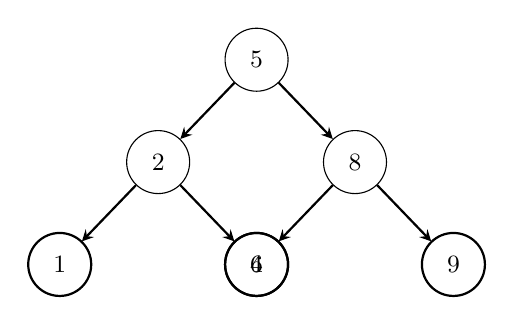
\begin{tikzpicture}[
  every node/.style={circle, draw, minimum size=0.8cm, font=\small, inner sep=1pt},
  level distance=1.3cm,
  sibling distance=2.5cm,
  edge from parent/.style={draw, ->, >=stealth, thick}
]
\node {5}
  child { node {2}
    child { node {1} }
    child { node {4} }
  }
  child { node {8}
    child { node {6} }
    child { node {9} }
  };
\end{tikzpicture}
\caption{A valid BST. Every node in the left subtree of 5 is $< 5$, and every node in the right subtree is $> 5$. This property holds recursively at every node.}
\end{figure}

%% ============================================================
\section{Search in BST}
\label{sec:search}

\subsection{Algorithm}

The BST ordering invariant enables binary-search-style elimination: at each node, we either find the target, or eliminate one entire subtree:

\begin{verbatim}
boolean search(TreeNode root, int target) {
    if (root == null) return false;
    
    if (root.data == target) return true;
    
    if (target < root.data) {
        return search(root.left, target);
    } else {
        return search(root.right, target);
    }
}
\end{verbatim}

\begin{theorem}[Search Correctness]
If $v$ exists in BST $T$, then \texttt{search(T.root, v)} returns \texttt{true}. If $v$ does not exist, it returns \texttt{false}.
\end{theorem}

\begin{proof}
By structural induction on the tree height.

\textbf{Base case:} $\texttt{root} = \texttt{null}$. The target is not in the empty tree. Returns \texttt{false}. $\checkmark$

\textbf{Inductive step:} Assume correctness for trees of height $< h$. For a tree of height $h$:
\begin{itemize}
    \item If $\texttt{target} = \texttt{root.data}$, return \texttt{true}. $\checkmark$
    \item If $\texttt{target} < \texttt{root.data}$: by the BST property, the target (if it exists) must be in the left subtree. We recurse on \texttt{root.left}, which has height $< h$. By the inductive hypothesis, the result is correct. $\checkmark$
    \item If $\texttt{target} > \texttt{root.data}$: symmetrically, we recurse on \texttt{root.right}. $\checkmark$
\end{itemize}
\end{proof}

\subsection{Example and Dry Run}

\begin{figure}[htbp]
\centering
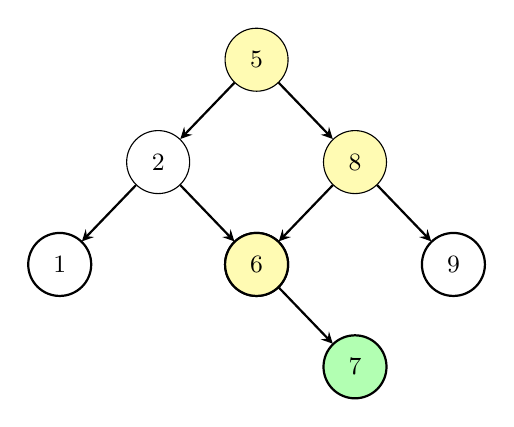
\begin{tikzpicture}[
  every node/.style={circle, draw, minimum size=0.8cm, font=\small, inner sep=1pt},
  level distance=1.3cm,
  sibling distance=2.5cm,
  edge from parent/.style={draw, ->, >=stealth, thick}
]
\node[fill=yellow!30] {5}
  child { node {2}
    child { node {1} }
    child { node {4} }
  }
  child { node[fill=yellow!30] {8}
    child { node[fill=yellow!30] {6}
      child[missing] {}
      child { node[fill=green!30] {7} }
    }
    child { node {9} }
  };
\end{tikzpicture}
\caption{Search path for $K=7$ (highlighted in yellow, target in green).}
\end{figure}

\textbf{Dry Run --- search(root, 7):}

\begin{table}[htbp]
\centering
\begin{tabular}{|c|c|c|c|}
\hline
\textbf{Step} & \textbf{Current Node} & \textbf{Comparison} & \textbf{Action} \\
\hline
1 & 5 & $7 > 5$ & Go right \\
2 & 8 & $7 < 8$ & Go left \\
3 & 6 & $7 > 6$ & Go right \\
4 & 7 & $7 = 7$ & \textbf{Return true} \\
\hline
\end{tabular}
\caption{Search trace for target $K=7$. Visited 4 nodes out of 7 total.}
\end{table}

\subsection{Complexity Analysis}

\begin{itemize}
    \item \textbf{Time:} $O(H)$ where $H$ is the height of the BST.
    \begin{itemize}
        \item Best case (balanced BST): $O(\log N)$
        \item Worst case (skewed BST): $O(N)$
    \end{itemize}
    \item \textbf{Space:} $O(H)$ for the recursion stack (can be reduced to $O(1)$ with iterative approach).
\end{itemize}

%% ============================================================
\section{Insertion in BST}
\label{sec:insert}

\subsection{Key Insight}

New nodes are always inserted as \emph{leaf nodes}. We traverse the tree using the BST property to find the correct position, then create a new node at the \texttt{null} position:

\begin{verbatim}
TreeNode insert(TreeNode root, int value) {
    if (root == null) {
        return new TreeNode(value);
    }
    
    if (value < root.data) {
        root.left = insert(root.left, value);
    } else if (value > root.data) {
        root.right = insert(root.right, value);
    }
    // If value == root.data, ignore (no duplicates)
    
    return root;
}
\end{verbatim}

\begin{theorem}[Insertion Correctness]
After \texttt{insert(root, value)}, the resulting tree is a valid BST containing all original elements plus the new value.
\end{theorem}

\begin{proof}
By structural induction.

\textbf{Base case:} $\texttt{root} = \texttt{null}$. We create a single-node tree with the given value. A single node is trivially a valid BST. $\checkmark$

\textbf{Inductive step:} If $\texttt{value} < \texttt{root.data}$, we insert into the left subtree. By the inductive hypothesis, the left subtree remains a valid BST containing the new value. Since $\texttt{value} < \texttt{root.data}$, the BST property at the root is preserved. The right subtree is unchanged. Symmetric argument applies for $\texttt{value} > \texttt{root.data}$. $\checkmark$
\end{proof}

\subsection{Example and Dry Run}

Insert value \textbf{6} into the following BST:

\begin{figure}[htbp]
\centering
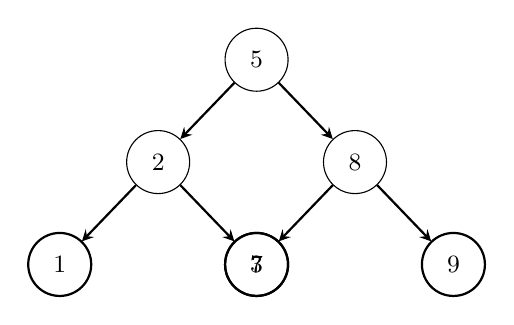
\begin{tikzpicture}[
  every node/.style={circle, draw, minimum size=0.8cm, font=\small, inner sep=1pt},
  level distance=1.3cm,
  sibling distance=2.5cm,
  edge from parent/.style={draw, ->, >=stealth, thick}
]
\node {5}
  child { node {2}
    child { node {1} }
    child { node {3} }
  }
  child { node {8}
    child { node {7} }
    child { node {9} }
  };
\end{tikzpicture}
\caption{BST before inserting 6.}
\end{figure}

\textbf{Dry Run --- insert(root, 6):}

\begin{table}[htbp]
\centering
\begin{tabular}{|c|c|c|c|}
\hline
\textbf{Step} & \textbf{Node} & \textbf{Comparison} & \textbf{Action} \\
\hline
1 & 5 & $6 > 5$ & Go right \\
2 & 8 & $6 < 8$ & Go left \\
3 & 7 & $6 < 7$ & Go left \\
4 & null & --- & Create node(6), return \\
\hline
\end{tabular}
\caption{Node 6 is inserted as the left child of node 7.}
\end{table}

\begin{figure}[htbp]
\centering
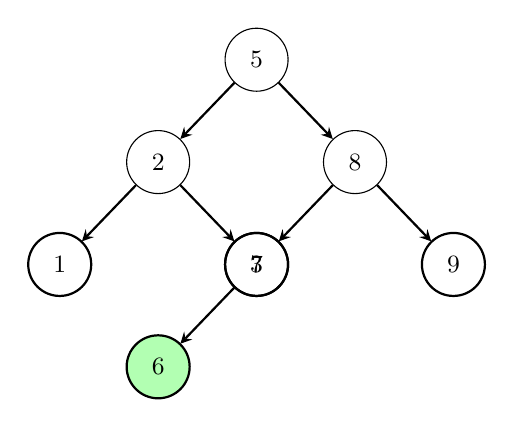
\begin{tikzpicture}[
  every node/.style={circle, draw, minimum size=0.8cm, font=\small, inner sep=1pt},
  level distance=1.3cm,
  sibling distance=2.5cm,
  edge from parent/.style={draw, ->, >=stealth, thick}
]
\node {5}
  child { node {2}
    child { node {1} }
    child { node {3} }
  }
  child { node {8}
    child { node {7}
      child { node[fill=green!30] {6} }
      child[missing] {}
    }
    child { node {9} }
  };
\end{tikzpicture}
\caption{BST after inserting 6 (highlighted in green).}
\end{figure}

\subsection{Complexity Analysis}

\begin{itemize}
    \item \textbf{Time:} $O(H)$ --- we traverse one path from root to a leaf.
    \item \textbf{Space:} $O(H)$ for recursion stack.
\end{itemize}

%% ============================================================
\section{Finding Minimum and Maximum}
\label{sec:minmax}

\subsection{Key Insight}

By the BST property:
\begin{itemize}
    \item The \textbf{smallest} element is the leftmost node (follow left pointers until null).
    \item The \textbf{largest} element is the rightmost node (follow right pointers until null).
\end{itemize}

\subsection{Algorithms}

\begin{verbatim}
TreeNode findMin(TreeNode root) {
    TreeNode temp = root;
    while (temp.left != null) {
        temp = temp.left;
    }
    return temp;
}

TreeNode findMax(TreeNode root) {
    TreeNode temp = root;
    while (temp.right != null) {
        temp = temp.right;
    }
    return temp;
}
\end{verbatim}

\begin{theorem}[Minimum Element]
In a BST, the minimum element is located at the leftmost node.
\end{theorem}

\begin{proof}
Let $v$ be the leftmost node (i.e., $v.\text{left} = \texttt{null}$). For any other node $u$ in the tree:
\begin{itemize}
    \item If $u$ is an ancestor of $v$, then $v$ is in the left subtree of $u$, so $v.\text{data} < u.\text{data}$.
    \item If $u$ is in the right subtree of any ancestor of $v$, then $u.\text{data}$ is greater than that ancestor, which is greater than $v.\text{data}$.
\end{itemize}
Therefore $v.\text{data} \leq u.\text{data}$ for all nodes $u$, making $v$ the minimum. $\checkmark$
\end{proof}

\subsection{Example}

\begin{figure}[htbp]
\centering
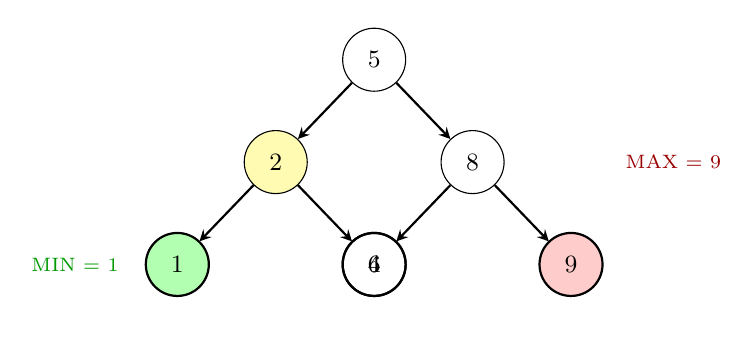
\begin{tikzpicture}[
  every node/.style={circle, draw, minimum size=0.8cm, font=\small, inner sep=1pt},
  level distance=1.3cm,
  sibling distance=2.5cm,
  edge from parent/.style={draw, ->, >=stealth, thick}
]
\node {5}
  child { node[fill=yellow!30] {2}
    child { node[fill=green!30] {1} }
    child { node {4} }
  }
  child { node {8}
    child { node {6} }
    child { node[fill=red!20] {9} }
  };

\node[draw=none, minimum size=0pt, font=\scriptsize, text=green!60!black] at (-3.8, -2.6) {MIN = 1};
\node[draw=none, minimum size=0pt, font=\scriptsize, text=red!60!black] at (3.8, -1.3) {MAX = 9};
\end{tikzpicture}
\caption{Minimum (leftmost, green) and Maximum (rightmost, red) in a BST.}
\end{figure}

\subsection{Complexity}

\begin{itemize}
    \item \textbf{Time:} $O(H)$ --- we follow one branch to a leaf.
    \item \textbf{Space:} $O(1)$ --- iterative, no recursion stack.
\end{itemize}

%% ============================================================
\section{Deletion in BST}
\label{sec:delete}

Deletion is the most complex BST operation because we must maintain the BST property after removing a node. There are three cases:

\subsection{Case 1: Deleting a Leaf Node}

The node has no children. Simply remove it by setting the parent's pointer to \texttt{null}.

\subsection{Case 2: Deleting a Node with One Child}

The node has exactly one child. Replace the node with its child (bypass the node).

\subsection{Case 3: Deleting a Node with Two Children}

This is the challenging case. We cannot simply remove the node. Instead:
\begin{enumerate}
    \item Find the \textbf{inorder successor} (smallest node in the right subtree) or the \textbf{inorder predecessor} (largest node in the left subtree).
    \item Copy the successor's value into the node to be deleted.
    \item Recursively delete the successor from the right subtree (which reduces to Case 1 or 2).
\end{enumerate}

\begin{theorem}[Inorder Successor Property]
The inorder successor of a node $v$ in a BST is the smallest value greater than $v.\text{data}$. It is always the leftmost node in the right subtree of $v$.
\end{theorem}

\subsection{Algorithm}

\begin{verbatim}
TreeNode delete(TreeNode root, int value) {
    if (root == null) return null;
    
    if (value < root.data) {
        root.left = delete(root.left, value);
    } else if (value > root.data) {
        root.right = delete(root.right, value);
    } else {
        // Found the node to delete
        
        // Case 1: Leaf node
        if (root.left == null && root.right == null) {
            return null;
        }
        
        // Case 2: One child
        if (root.left == null) return root.right;
        if (root.right == null) return root.left;
        
        // Case 3: Two children
        // Find inorder successor (min of right subtree)
        TreeNode successor = findMin(root.right);
        root.data = successor.data;
        root.right = delete(root.right, successor.data);
    }
    
    return root;
}
\end{verbatim}

\subsection{Example and Dry Run}

Delete node \textbf{5} (root) from the following BST:

\begin{figure}[htbp]
\centering
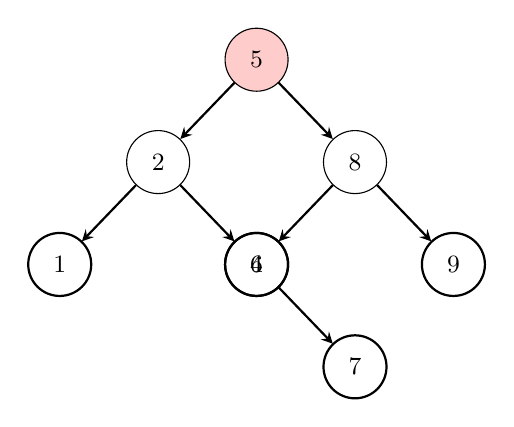
\begin{tikzpicture}[
  every node/.style={circle, draw, minimum size=0.8cm, font=\small, inner sep=1pt},
  level distance=1.3cm,
  sibling distance=2.5cm,
  edge from parent/.style={draw, ->, >=stealth, thick}
]
\node[fill=red!20] {5}
  child { node {2}
    child { node {1} }
    child { node {4} }
  }
  child { node {8}
    child { node {6}
      child[missing] {}
      child { node {7} }
    }
    child { node {9} }
  };
\end{tikzpicture}
\caption{BST before deleting root node 5. This is Case 3 (two children).}
\end{figure}

\textbf{Dry Run:}
\begin{enumerate}
    \item Node 5 has two children $\Rightarrow$ Case 3.
    \item Find inorder successor: smallest in right subtree of 5 = leftmost of subtree rooted at 8 = \textbf{6}.
    \item Copy 6 into node 5's position: root becomes 6.
    \item Recursively delete 6 from the right subtree. Node 6 has one child (7) $\Rightarrow$ Case 2. Replace 6 with 7.
\end{enumerate}

\begin{figure}[htbp]
\centering
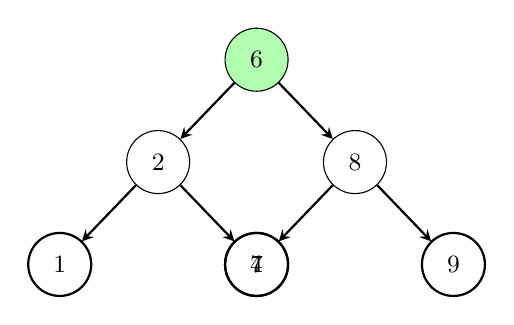
\begin{tikzpicture}[
  every node/.style={circle, draw, minimum size=0.8cm, font=\small, inner sep=1pt},
  level distance=1.3cm,
  sibling distance=2.5cm,
  edge from parent/.style={draw, ->, >=stealth, thick}
]
\node[fill=green!30] {6}
  child { node {2}
    child { node {1} }
    child { node {4} }
  }
  child { node {8}
    child { node {7} }
    child { node {9} }
  };
\end{tikzpicture}
\caption{BST after deleting 5. The inorder successor (6) replaced 5, and the original 6 was removed.}
\end{figure}

\subsection{Correctness Proof}

\begin{theorem}[Deletion Correctness]
After \texttt{delete(root, value)}, the resulting tree is a valid BST containing all original elements except the deleted value.
\end{theorem}

\begin{proof}
We prove each case:

\textbf{Case 1 (Leaf):} Removing a leaf does not affect any other node's BST relationships. $\checkmark$

\textbf{Case 2 (One child):} Bypassing a node with one child preserves the BST property because the child's entire subtree was already on the correct side of the deleted node's parent. $\checkmark$

\textbf{Case 3 (Two children):} The inorder successor $s$ is the smallest value in the right subtree. Replacing the deleted node's value with $s.\text{data}$ preserves the BST property because:
\begin{itemize}
    \item $s.\text{data}$ is greater than all values in the left subtree (since $s$ was in the right subtree and the original node's value was also greater).
    \item $s.\text{data}$ is less than all other values in the right subtree (since $s$ is the minimum of the right subtree).
    \item Recursively deleting $s$ from the right subtree reduces to Case 1 or 2 (since $s$, being the leftmost node, has no left child). $\checkmark$
\end{itemize}
\end{proof}

\subsection{Complexity Analysis}

\begin{itemize}
    \item \textbf{Time:} $O(H)$ --- at most two root-to-leaf traversals (one to find the node, one to find/delete the successor).
    \item \textbf{Space:} $O(H)$ for the recursion stack.
\end{itemize}

%% ============================================================
\section{Constructing a Balanced BST from a Sorted Array}
\label{sec:construct}

\subsection{Problem Statement}

Given a sorted array $A[0..N-1]$, construct a height-balanced BST containing all elements of $A$.

\subsection{Key Insight}

The middle element of the sorted array becomes the root. This ensures an approximately equal number of elements in the left and right subtrees, achieving minimum height:

\begin{verbatim}
TreeNode sortedArrayToBST(int[] A, int lo, int hi) {
    if (lo > hi) return null;
    
    int mid = lo + (hi - lo) / 2;
    TreeNode root = new TreeNode(A[mid]);
    
    root.left = sortedArrayToBST(A, lo, mid - 1);
    root.right = sortedArrayToBST(A, mid + 1, hi);
    
    return root;
}
\end{verbatim}

\begin{theorem}[Balanced Construction]
The tree produced by \texttt{sortedArrayToBST} is a valid BST with height $\lceil \log_2(N+1) \rceil - 1$, which is the minimum possible height for $N$ nodes.
\end{theorem}

\begin{proof}
\textbf{BST Property:} Since $A$ is sorted, $A[\text{lo}..mid-1] < A[\text{mid}] < A[mid+1..\text{hi}]$. The left subtree contains only elements less than the root, and the right subtree contains only elements greater. By induction, each subtree is also a valid BST. $\checkmark$

\textbf{Balance:} At each level, the array is divided into two halves differing in size by at most 1. This produces a tree where every node's subtree heights differ by at most 1. $\checkmark$
\end{proof}

\subsection{Example}

\textbf{Input:} $A = [1, 2, 3, 4, 5, 6, 7]$

\begin{table}[htbp]
\centering
\begin{tabular}{|c|c|c|c|}
\hline
\textbf{Call} & \textbf{Range [lo, hi]} & \textbf{mid} & \textbf{Root Value} \\
\hline
1 & [0, 6] & 3 & 4 \\
2 & [0, 2] & 1 & 2 \\
3 & [0, 0] & 0 & 1 (leaf) \\
4 & [2, 2] & 2 & 3 (leaf) \\
5 & [4, 6] & 5 & 6 \\
6 & [4, 4] & 4 & 5 (leaf) \\
7 & [6, 6] & 6 & 7 (leaf) \\
\hline
\end{tabular}
\caption{Recursive construction trace for $A = [1,2,3,4,5,6,7]$.}
\end{table}

\begin{figure}[htbp]
\centering
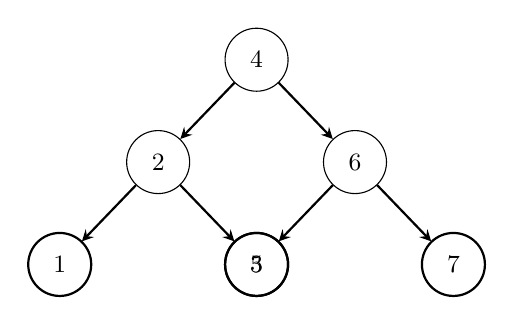
\begin{tikzpicture}[
  every node/.style={circle, draw, minimum size=0.8cm, font=\small, inner sep=1pt},
  level distance=1.3cm,
  sibling distance=2.5cm,
  edge from parent/.style={draw, ->, >=stealth, thick}
]
\node {4}
  child { node {2}
    child { node {1} }
    child { node {3} }
  }
  child { node {6}
    child { node {5} }
    child { node {7} }
  };
\end{tikzpicture}
\caption{Balanced BST constructed from sorted array $[1,2,3,4,5,6,7]$. Height $= 2 = \lceil\log_2 8\rceil - 1$.}
\end{figure}

\subsection{Complexity}

\begin{itemize}
    \item \textbf{Time:} $O(N)$ --- each element is visited exactly once.
    \item \textbf{Space:} $O(\log N)$ --- recursion depth equals tree height (balanced).
\end{itemize}

%% ============================================================
\section{BST Validation}
\label{sec:validate}

We present two approaches to verify whether a given binary tree satisfies the BST property.

\subsection{Approach 1: Inorder Traversal Check}

\begin{lemma}[Inorder Property of BSTs]
The inorder traversal of a valid BST produces elements in strictly increasing (sorted) order.
\end{lemma}

\begin{verbatim}
boolean isBSTInorder(TreeNode root) {
    List<Integer> result = new ArrayList<>();
    inorder(root, result);
    
    for (int i = 1; i < result.size(); i++) {
        if (result.get(i) <= result.get(i - 1)) {
            return false;
        }
    }
    return true;
}

void inorder(TreeNode root, List<Integer> result) {
    if (root == null) return;
    inorder(root.left, result);
    result.add(root.data);
    inorder(root.right, result);
}
\end{verbatim}

\textbf{Complexity:} $O(N)$ time, $O(N)$ space (for storing the traversal).

\subsection{Approach 2: Min-Max Range Validation}

A more elegant approach passes valid value ranges down the recursion:

\begin{verbatim}
boolean isBST(TreeNode root, int min, int max) {
    if (root == null) return true;
    
    if (root.data <= min || root.data >= max) {
        return false;
    }
    
    boolean leftValid = isBST(root.left, min, root.data);
    boolean rightValid = isBST(root.right, root.data, max);
    
    return leftValid && rightValid;
}

// Initial call:
// isBST(root, Integer.MIN_VALUE, Integer.MAX_VALUE)
\end{verbatim}

\begin{theorem}[Range Validation Correctness]
\texttt{isBST(v, min, max)} returns \texttt{true} if and only if all values in the subtree rooted at $v$ lie in the open interval $(\text{min}, \text{max})$ and the subtree satisfies the BST property.
\end{theorem}

\begin{proof}
By structural induction.

\textbf{Base case:} $v = \texttt{null}$. Returns \texttt{true}. An empty tree trivially satisfies any range constraint. $\checkmark$

\textbf{Inductive step:} 
\begin{itemize}
    \item If $v.\text{data} \leq \text{min}$ or $v.\text{data} \geq \text{max}$, the value is out of the valid range. Return \texttt{false}. $\checkmark$
    \item For the left subtree: all values must be in $(\text{min}, v.\text{data})$. The recursive call \texttt{isBST(v.left, min, v.data)} enforces this. $\checkmark$
    \item For the right subtree: all values must be in $(v.\text{data}, \text{max})$. The recursive call \texttt{isBST(v.right, v.data, max)} enforces this. $\checkmark$
\end{itemize}
\end{proof}

\subsection{Dry Run of Min-Max Approach}

\begin{figure}[htbp]
\centering
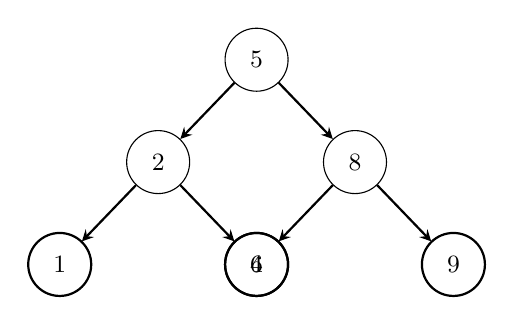
\begin{tikzpicture}[
  every node/.style={circle, draw, minimum size=0.8cm, font=\small, inner sep=1pt},
  level distance=1.3cm,
  sibling distance=2.5cm,
  edge from parent/.style={draw, ->, >=stealth, thick}
]
\node {5}
  child { node {2}
    child { node {1} }
    child { node {4} }
  }
  child { node {8}
    child { node {6} }
    child { node {9} }
  };
\end{tikzpicture}
\caption{Valid BST for min-max validation dry run.}
\end{figure}

\begin{table}[htbp]
\centering
\begin{tabular}{|c|c|c|c|c|}
\hline
\textbf{Node} & \textbf{min} & \textbf{max} & \textbf{Valid?} & \textbf{Action} \\
\hline
5 & $-\infty$ & $+\infty$ & $-\infty < 5 < +\infty$ $\checkmark$ & recurse \\
2 & $-\infty$ & 5 & $-\infty < 2 < 5$ $\checkmark$ & recurse \\
1 & $-\infty$ & 2 & $-\infty < 1 < 2$ $\checkmark$ & leaf, true \\
4 & 2 & 5 & $2 < 4 < 5$ $\checkmark$ & leaf, true \\
8 & 5 & $+\infty$ & $5 < 8 < +\infty$ $\checkmark$ & recurse \\
6 & 5 & 8 & $5 < 6 < 8$ $\checkmark$ & leaf, true \\
9 & 8 & $+\infty$ & $8 < 9 < +\infty$ $\checkmark$ & leaf, true \\
\hline
\end{tabular}
\caption{Min-max validation trace. All nodes pass $\Rightarrow$ \textbf{Valid BST}.}
\end{table}

\subsection{Complexity Comparison}

\begin{table}[htbp]
\centering
\begin{tabular}{|l|c|c|}
\hline
\textbf{Approach} & \textbf{Time} & \textbf{Space} \\
\hline
Inorder traversal + sorted check & $O(N)$ & $O(N)$ \\
Min-Max range validation & $O(N)$ & $O(H)$ \\
\hline
\end{tabular}
\caption{The min-max approach is superior in space complexity.}
\end{table}

%% ============================================================
\section{Comprehensive Complexity Summary}
\label{sec:summary}

\begin{table}[htbp]
\centering
\begin{tabular}{|l|c|c|c|}
\hline
\textbf{Operation} & \textbf{Average} & \textbf{Worst} & \textbf{Space} \\
\hline
Search & $O(\log N)$ & $O(N)$ & $O(H)$ \\
Insert & $O(\log N)$ & $O(N)$ & $O(H)$ \\
Find Min/Max & $O(\log N)$ & $O(N)$ & $O(1)$ \\
Delete & $O(\log N)$ & $O(N)$ & $O(H)$ \\
Sorted Array to BST & $O(N)$ & $O(N)$ & $O(\log N)$ \\
Validate (Inorder) & $O(N)$ & $O(N)$ & $O(N)$ \\
Validate (Min-Max) & $O(N)$ & $O(N)$ & $O(H)$ \\
\hline
\end{tabular}
\caption{Complete BST operations complexity summary. $H$ = tree height, ranging from $O(\log N)$ (balanced) to $O(N)$ (skewed).}
\end{table}

\subsection{BST vs. Balanced BST Variants}

\begin{table}[htbp]
\centering
\begin{tabular}{|l|c|c|c|}
\hline
\textbf{Data Structure} & \textbf{Search} & \textbf{Insert} & \textbf{Delete} \\
\hline
Unbalanced BST & $O(N)$ worst & $O(N)$ worst & $O(N)$ worst \\
AVL Tree & $O(\log N)$ & $O(\log N)$ & $O(\log N)$ \\
Red-Black Tree & $O(\log N)$ & $O(\log N)$ & $O(\log N)$ \\
\hline
\end{tabular}
\caption{Motivation for self-balancing BST variants.}
\end{table}

\section{Conclusion}

This paper presented a comprehensive formal analysis of seven fundamental Binary Search Tree operations: search, insertion, finding minimum/maximum, deletion (all three cases), balanced BST construction from sorted arrays, and BST validation via both inorder traversal and min-max range checking.

Key takeaways include:
\begin{itemize}
    \item \textbf{Search/Insert/Delete:} All follow the same pattern of traversing one root-to-leaf path, achieving $O(H)$ time. The BST ordering invariant enables efficient binary-search-style elimination at each step.
    \item \textbf{Deletion Case 3:} The most subtle operation --- replacing a two-child node with its inorder successor (or predecessor) elegantly reduces to simpler deletion cases while preserving the BST property.
    \item \textbf{Sorted Array to BST:} The divide-and-conquer approach of always choosing the middle element produces an optimally balanced tree in $O(N)$ time.
    \item \textbf{BST Validation:} The min-max range approach is superior to the inorder traversal method, requiring only $O(H)$ space versus $O(N)$, and operates in a single pass without materializing the full traversal.
    \item \textbf{Height Sensitivity:} All BST operations are $O(H)$, making tree balance critical. An unbalanced BST degenerates to $O(N)$ operations, motivating self-balancing variants like AVL trees and Red-Black trees.
\end{itemize}

\begin{thebibliography}{10}
\bibitem{cormen} T.~H.~Cormen, C.~E.~Leiserson, R.~L.~Rivest, and C.~Stein, \emph{Introduction to Algorithms}, 4th~ed. MIT Press, 2022.
\bibitem{knuth} D.~E.~Knuth, \emph{The Art of Computer Programming, Volume 3: Sorting and Searching}, 2nd~ed. Addison-Wesley, 1998.
\bibitem{sedgewick} R.~Sedgewick and K.~Wayne, \emph{Algorithms}, 4th~ed. Addison-Wesley, 2011.
\bibitem{skiena} S.~S.~Skiena, \emph{The Algorithm Design Manual}, 3rd~ed. Springer, 2020.
\bibitem{adelson} G.~M.~Adelson-Velsky and E.~M.~Landis, ``An algorithm for the organization of information,'' \emph{Soviet Mathematics Doklady}, vol.~3, pp.~1259--1263, 1962.
\bibitem{guibas} L.~J.~Guibas and R.~Sedgewick, ``A dichromatic framework for balanced trees,'' in \emph{Proc.\ 19th Annual IEEE FOCS}, pp.~8--21, 1978.
\bibitem{hibbard} T.~N.~Hibbard, ``Some combinatorial properties of certain trees with applications to searching and sorting,'' \emph{Journal of the ACM}, vol.~9, no.~1, pp.~13--28, 1962.
\end{thebibliography}


\end{document}
